\chapter{Technical preliminaries}\label{semantics}

In this chapter we will introduce the technical preliminaries used throughout
this paper. We begin by giving the definitions of modal, doxastic and epistemic
logics that we use. We then introduce the concept of a refinement, and then
define the syntax and semantics of the refinement quantified modal logics
themselves.

\section{Modal, doxastic and epistemic logics}

In this section we recall the definitions of modal, doxastic and epistemic
logics, and the notation that we use for these logics. We refer the reader to
Appendix~\ref{modal} for a more thorough introduction to modal logics.

% Definition of Kripke models
Let $A$ be a non-empty, finite set of agents, and let $P$ be a non-empty,
countable set of propositional atoms.

\begin{definition}[Kripke model]
A \textit{Kripke model} $M = (S, R, V)$ consists of a \textit{domain} $S$, which
is a set of states (or worlds), \textit{accessibility} $R : A \to \mathcal{P}(S
\times S)$, and a \textit{valuation} $V : P \to \mathcal{P}(S)$. 

The class of all Kripke models is called \classK{}. We write $M \in \classK{}$
to denote that $M$ is a Kripke model.
\end{definition}

For $R(a)$, we write $R_a$. We write $sR_a$ for $\{t \mid (s, t) \in R_a\}$ and
we write $R_at$ for $\{s \mid (s, t) \in R_a\}$. As we will be required to
discuss several models at once, we will use the convention that $M = (S^M, R^M,
V^M)$, $N = (S^N, R^N, V^N)$, and so on. For $s \in S^M$ we will let $M_s$ refer
to the pair $(M, s)$, also known as the pointed Kripke model of $M$ at state
$s$.

\begin{definition}[Doxastic model]
A \textit{doxastic model} is a Kripke model $M = (S, R, V)$ such that the
relation $R_a$ is serial, transitive, and Euclidean for all $a \in A$. The class
of all doxastic models is called \classKD{}. We write $M \in \classKD{}$ to
denote that $M$ is a doxastic model.
\end{definition}

\begin{definition}[Epistemic model]
An \textit{epistemic model} is a Kripke model $M = (S, R, V)$ such that the
relation $R_a$ is an equivalence relation for all $a \in A$. The class of all
epistemic models is called \classS{}. We write $M \in \classS{}$ to denote that
$M$ is an epistemic model.
\end{definition}

Throughout this paper we will be presenting results in both doxastic and
epistemic logic.  As such, when we are discussing doxastic logic, we will
assume that all Kripke models are implicitly doxastic models, and likewise when
we are discussing epistemic logic, we will assume that all Kripke models are
implicitly epistemic models. When we are discussing results in general modal
logic, we will not assume any restrictions on the Kripke models.

% Syntax of modal logics
\begin{definition}[Language of \lang{}]
Given a non-empty, finite set of agents $A$ and a non-empty, countable set of
propositional atoms $P$, the language of \lang{} is defined by the following
abstract syntax:
$$
\alpha ::=  p \bnfalt
            \neg \alpha \bnfalt
            \alpha \land \alpha \bnfalt
            \knows_a \alpha
$$
where $p \in P$, $a \in A$ and $\alpha \in \lang{}$.
\end{definition}

Standard abbreviations include:
$\top ::= p \lor \neg p$;
$\bot ::= \neg \top$;
$\phi \lor \psi ::= \neg (\neg \phi \land \neg \psi)$;
$\phi \implies \psi ::= \neg \phi \lor \psi$;
and $\suspects_a \phi ::= \neg \knows_a \neg \phi$.

We also use the cover operator $\covers_a \Gamma$, where $\Gamma$ is a finite
set of formulae, which is an abbreviation for $\covers_a \Gamma ::= \knows_a
\bigvee_{\gamma \in \Gamma} \gamma \land \bigwedge_{\gamma \in \Gamma}
\suspects_a \gamma$. An axiomatisation of the modal $\mu$-calculus, using the
cover operator, was given by Bilkova, Palmigiano and
Venema~\cite{bilkova2008proof}. The cover operator is relied on for our
axiomatisation, in much the same way it is relied on for the axiomatisation of
\logicKiF{} presented by van Ditmarsch, French and
Pinchinat~\cite{french2010future}.

We note that the basic modalities $\knows_a$ and $\suspects_a$ can be expressed
in terms of the cover operator, a fact that we will rely upon for all of our
axiomatisations. We note that $\knows_a \phi \iff \covers_a \{\phi\} \lor
\covers_a \emptyset$ and $\suspects_a \phi \iff \covers_a \{\phi,
\top\}$~\cite{bilkova2008proof}. 

% Semantics of modal logics
\begin{definition}[Semantics of \logicC{}]
Let \classC{} be a class of Kripke models, and let $M = (S, R, V) \in \classC$
be a Kripke model taken from \classC{}. The interpretation of $\phi$ is defined
inductively:
\begin{eqnarray*}
M_s &\entails& p \text{ iff } s \in V_p\\
M_s &\entails& \neg \phi \text{ iff } M_s \nentails \phi\\
M_s &\entails& \phi \land \psi \text{ iff } M_s \entails \phi \text{ and } M_s
\entails \psi\\
M_s &\entails& \knows_a \phi \text{ if for all } t \in S : (s, t) \in R_a \text{
implies } M_t \entails \phi
\end{eqnarray*}
\end{definition}

We say that a formula $\phi$ is {\em satisfied} by a pointed Kripke model $M_s
\in \classC$ if and only if $M_s \entails \phi$. We say that $\phi$ is satisfied
by a Kripke model $M \in \classC$ if and only if $M_s \entails \phi$ for some $s
\in S^M$. We say that $\phi$ is {\em satisfied} by a class of Kripke models
$\classC$ if and only if it is satisfied by every Kripke model $M \in \classC$.
We say that $\phi$ is {\em valid} in a Kripke model $M \in \classC$ if and only
if $M_s \entails \phi$ for every $s \in S^M$. We write $M \entails \phi$. We say
that $\phi$ is {\em valid} in a class of Kripke models $\classC$ if and only if
$M \entails \phi$ for every $M \in \classC$. We write $\classC \entails \phi$.

The logics \logicK{}, \logicKD{} and \logicS{} are instances of \logicC{} with
classes \classK{}, \classKD{} and \classS{} respectively. It should be noted
that \logicKD{} is a conservative extension of \logicK{}, and \logicS{} is a
conservative extension of \logicKD{} (and also of \logicK{}). This means that
every valid formula in \logicK{} is also valid in \logicKD{}, and likewise for
\logicKD{} and \logicS{}. This is because any formula that is valid with respect
to a particular class of Kripke models is also valid for any subclass of those
Kripke models.

\section{Bisimulation, simulation and refinements}

In this section we introduce refinements, the concept that is central to the
refinement quantified modal logics. We first introduce the related notion of a
bisimulation, and define simulations and refinements in terms of the properties
that define a bisimulation. We finally remark on the properties of refinements
that make them suitable for representing informative updates in the refinement
quantified modal logics.

\begin{definition}[Bisimulation]
Let $M = (S, R, V)$ and $M' = (S', R', V')$ be Kripke models. A non-empty
relation $\mathcal{R} \subseteq S \times S'$ is a \textit{bisimulation} if and
only if for all $s \in S$ and $s' \in S'$, with $(s, s') \in \mathcal{R}$, for
all $a \in A$:

\begin{description}
\item[atoms] $s \in V(p)$ if and only if $s' \in V'(p)$ for all
$p \in P$

\item[forth-$a$] for all $t \in S$, if $R_a(s, t)$, then there is a
$t' \in S'$ such that $R'_a(s', t')$ and $(t,
t') \in \mathcal{R}$

\item[back-$a$] for all $t' \in S'$, if $R'_a(s',
t')$, then there is a $t \in S$ such that $R_a(s, t)$ and $(t, t')
\in \mathcal{R}$.
\end{description}

We call $M_s$ and $M'_{s'}$ bisimilar, and write $M_s \bisim M'_{s'}$ to denote
that there is a bisimulation between $M_s$ and $M'_{s'}$.
\end{definition}

We note that bisimulation is an equivalence relation.

Bisimulations relate Kripke models that are in a sense indistinguishable to
modal logics. If two Kripke models are bisimilar, then they each satisfy the
same set of modal formulae. This is a property of modal logics that is called
bisimulation invariance.

\begin{lemma}
Let $M_s, M'_{s'} \in \classK$ be Kripke models such that $M_s \bisim M'_{s'}$,
and let $\phi \in \lang$. Then $M_s \entails \phi$ if and only if $M'_{s'}
\entails \phi$.
\end{lemma}

This is shown by Blackburn, de Rijke and Venema~\cite{blackburn2002modal}. We
note that this result holds equally if the models $M_s$ and $M'_{s'}$ are taken
from subclasses of \classK{}.

If we relax the properties of bisimulation slightly, we get a related notion
known as a {\em simulation}, or its reverse relation, a {\em refinement}.

\begin{definition}[Simulation and refinement]
Let $M$ and $M'$ be Kripke models. A non-empty relation $\mathcal{R}
\subseteq S \times S'$ is a \textit{simulation} if and only if it satisfied {\bf
atoms} and {\bf forth-$a$} for every $a \in A$.

We call $M'_{s'}$ a simulation of $M_s$ and we call $M_s$ a refinement of
$M'_{s'}$. We write $M'_{s'} \simulation M_s$ to denote this, or alternatively,
$M_s \refinement M'_{s'}$.

A relation that satisfies {\bf atoms} and {\bf forth-$b$} for every $b \in A$,
and satisfies {\bf back-$b$} for every $b \in A - \{a\}$, for some $a \in A$, is
an $a$\textit{-simulation}. 

We call $M'_{s'}$ an $a$-simulation of $M_s$, and we call $M_s$ an
$a$-refinement of $M'_{s'}$. We write $M'_{s'} \simulation_a M_s$ to denote
this, or alternatively, $M_s \refinement_a M'_{s'}$.
\end{definition}

\begin{lemma}\label{semantics-preorder}
The relation $\refinement_a$ is reflexive and transitive, and satisfies the
Church-Rosser property over the class of \classK{} models.
\end{lemma}

This is shown by van Ditmarsch and French~\cite{french2009simulation}

As we have mentioned before, refinement quantified modal logics quantify over
informative updates, by quantifying over the refinements of a Kripke model. We
will briefly introduce two properties to illustrate how refinements correspond
to the notion of an informative update.

\begin{definition}[Positive formulae]
A positive formula is defined by the following abstract syntax:
$$
\alpha ::=    p \bnfalt 
            \neg p \bnfalt
            \alpha \land \alpha \bnfalt
            \alpha \lor \alpha \bnfalt
            \knows_a \alpha
$$
where $p \in P$ and $a \in A$.
\end{definition}

\begin{proposition}\label{pre-positive}
Let $M_s$ and $M'_{s'}$ be Kripke models such that $M'_{s'} \refinement M_s$,
and let $\phi$ be a positive formula. If $M_s \entails \phi$ then $M'_{s'}
\entails \phi$. 
\end{proposition}

Using an epistemic interpretation, one can reasonably say that an informative
update should only cause an agent to gain additional information, and cannot
cause an agent to {\em forget} any information that it has previously been told.
Thus anything that an agent knows before an informative update, the agent should
continue to know after an informative update. This is not quite accurate, as a
formula that involves {\em negative knowledge} may be invalidated by an
informative update. For example, suppose that we have a situation where
$\knows_a \neg \knows_b p$, i.e. $a$ knows that $b$ doesn't know that $p$. We
say this situation involves negative knowledge because it refers to a lack of
knowledge of agent $b$. Then it is reasonable that an informative update could
tell $b$ that $p$ is true, and so after the informative update, $\knows_b p$
becomes true.  This causes $\neg \knows_b p$ to become false, and since it is
now false, it cannot possibly be known, since only true statements can be
known. Thus not all knowledge is retained by an informative update, only
positive knowledge is retained. The fact that refinements preserve positive
knowledge is an important property for refinements in modelling informative
updates in an epistemic setting.

\begin{proposition}
On finite epistemic models, every finite refinement is equivalent to the
execution an action model.
\end{proposition}

This is shown by van Ditmarsch and French~\cite{french2009simulation}.

The property that every finite refinements is equivalent to the execution of an
action model is the main justification for refinements as representations of
informative updates. Although we do not explicitly define action models in this
paper, it should be noted that action models are inherently finite structures,
whereas the refinements of even a finite model can potentially be infinite, and
therefore the above property does not hold for the infinite refinements of
epistemic models. However van Ditmarsch and French~\cite{french2009simulation}
show that if the refinement quantified epistemic logic is extended with the
operator for reasoning about the results of specific action models, then the
resulting logic is equivalent to the arbitrary action model logic. Hence
quantifying over the refinements of a model is equivalent to quantifying over
the informative updates.

\section{Refinement quantified modal logics}

In this section we introduce the syntax and semantics of the refinement
quantified modal logics. The definitions that we give are general, in the sense
that the refinement quantified modal, doxastic and epistemic logics are all
instances of the definition that we give. We also provide some examples and
basic results that have previously been given by van Ditmarsch, French and
Pinchinat~\cite{french2010future}.

We begin with a definition of the language, \langF{}, of the refinement
quantified modal logics, along with a definition of its semantics over a general
class of frames.

\begin{definition}[Language of \langF{}]
Given a finite set of agents $A$ and a set of propositional atoms $P$, the
language of \langF{} is defined by the following abstract syntax:
$$
\alpha ::=  p \bnfalt
            \neg \alpha \bnfalt
            \alpha \land \alpha \bnfalt
            \knows_a \alpha \bnfalt
            \allrefs_a \alpha
$$
where $p \in P$, $a \in A$ and $\alpha \in \lang{}$.
\end{definition}

We use the standard abbreviations from basic modal logic, along with an
abbreviation for the dual of the $\allrefs_a$ operator, $\somerefs_a \phi ::=
\neg \allrefs_a \neg \phi$.

\begin{definition}[Semantics of \logicCF{}]
Let \classC{} be a class of Kripke models, and let $M = (S, R, V) \in \classC$
be a Kripke model taken from \classC{}. The interpretation of $\phi$ is defined
inductively.
\begin{eqnarray*}
M_s &\entails& p \text{ iff } s \in V_p\\
M_s &\entails& \neg \phi \text{ iff } M_s \nentails \phi\\
M_s &\entails& \phi \land \psi \text{ iff } M_s \entails \phi \text{ and } M_s
\entails \psi\\
M_s &\entails& \knows_a \phi \text{ if for all } t \in S : (s, t) \in R_a \text{
implies } M_t \entails \phi\\
M_s &\entails& \allrefs_a \phi \text{ iff for all } M'_{s'} \in \classC : M_s
\simulation_a M'_{s'} \text{ implies } M'_{s'} \entails \phi
\end{eqnarray*}
\end{definition}

We use the same terminology and notation for satisfiability and validity as is
used for basic modal logics. As we sometimes discuss basic modal logics and
refinement quantified modal logics at the same time, we may add a subscript to
the turnstile operator, e.g. $\entails_\somerefs \phi$, to make it
explicit that we are working in the refinement quantified version of the logic.

The logics \logicKF{}, \logicKDF{} and \logicSF{} are instances of \logicCF{},
with classes \classK{}, \classKD{} and \classS{} respectively. 

It should be emphasised that the interpretation of the refinement quantifier,
$\allrefs_a$, varies for each logic, as the refinements considered in the
interpretation of each logic must be taken from the appropriate class of Kripke
models. It is for this reason that \logicSF{} and \logicKDF{} are not
conservative extensions of \logicKF{}. For example, $\somerefs_a \knows_a \bot$
is valid in \logicKF{}, but not in \logicSF{} or \logicKDF{}. This is because
given any pointed model in \classK{}, one can construct an $a$-refinement from
that model by deleting the $a$-edges starting at the designated state; in this
resulting $a$-refinement, $\knows_a \bot$ is satisfied, and hence $\somerefs_a
\knows_a \bot$ is satisfied in the original model. However because of the serial
property of \classS{} and \classKD{} models, $\knows_a \bot$ is not even
satisfiable in \logicSF{} or \logicKDF{}, and hence $\somerefs_a \knows_a \bot$
is not satisfiable either, as the refinement required must be taken from the
classes of \classS{} or \classKD{}.

We also note that for a class of frames \classC{}, the refinement quantified
modal logic \logicCF{} is a conservative extension of the basic modal logic
\logicC{}. This is because the interpretation of any formula that does not
contain a $\allrefs_a$ operator is the same as the interpretation of that
formula in basic modal logic.

\begin{lemma}
The logic \logicKF{} is bisimulation invariant.
\end{lemma}

This is proven by van Ditmarsch, French and Pinchinat~\cite{french2010future}.

\begin{lemma}
The logics \logicKDF{} and \logicSF{} are bisimulation invariant.
\end{lemma}

The proof for bisimulation invariance in \logicKF{}, given by van Ditmarsch,
French and Pinchinat~\cite{french2010future} applies to \logicSF{} and
\logicKDF{}.

% Examples
\begin{example}\label{semantics-coin-s5}
We recall the coin-flipping example previously given in
Section~\ref{litreview-am}.  Suppose that Alice has flipped a coin, and
initially Alice and Bob do not know whether the coin landed on heads or tails,
and that both Alice and Bob are aware of each other's ignorance of the result.
We represent Alice by the symbol $a$, Bob by the symbol $b$, the result that the
coin landed on heads by the propositional atom $p$, and the result that the coin
landed on tails by the negated atom, $\neg p$. This situation can be represented
by the epistemic model in Figure~\ref{semantics-coin-s5-1}.

\begin{figure}
\begin{center} 
\scalebox{0.4}{
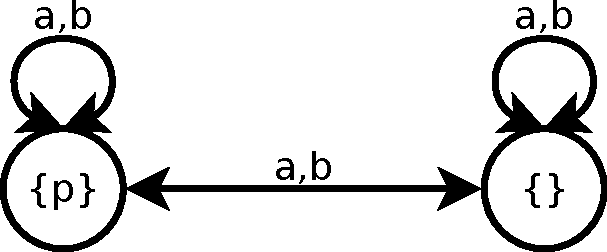
\includegraphics{semantics-coin-s5-1}
}
\caption{\label{semantics-coin-s5-1}
Initially Alice and Bob cannot distinguish between the worlds where the coin
lands on heads or on tails.
}
\end{center}
\end{figure}

Suppose that the coin actually landed on heads. Then the world where $p$ is true
is the actual world. We ask whether it is possible for Alice to learn that the
coin landed on heads whilst Bob continues to be ignorant of the result. We can
represent this question by the following statement in refinement quantified
epistemic logic:
$$\somerefs_a (\knows_a p \land \neg \knows_b p)$$ 

We can show that this statement is satisfied in the actual world of the above
epistemic model, by giving the $a$-refinement in Figure~\ref{semantics-coin-s5-2}

\begin{figure}
\begin{center} 
\scalebox{0.4}{
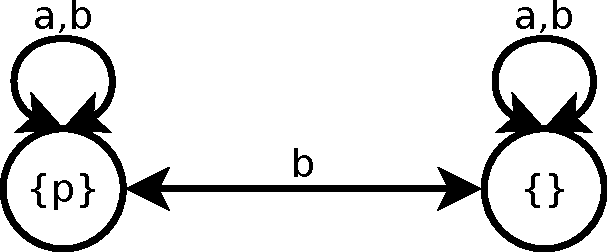
\includegraphics{semantics-coin-s5-2}
}
\caption{\label{semantics-coin-s5-2}
After Alice looks at the coin, she can distinguish between the worlds where the
coin lands on heads or tails, but Bob still cannot.
}
\end{center}
\end{figure}
\end{example}

\begin{example}\label{semantics-coin-kd45}
We recall the coin-flipping example again, but this time in the setting of
doxastic logic. We ask whether it is possible for Alice to learn that the coin
landed on heads whilst Bob continues to believe that Alice is ignorant of the
result. We can represent this question by the following statement in refinement
quantified doxastic logic:
$$\somerefs_a (\knows_a p \land \knows_b (\neg \knows_a p \land \neg \knows_a
\neg p))$$

We can show that this statement is satisfied by the model given in
Figure~\ref{semantics-coin-s5-1} by giving the $a$-refinement of the
model in Figure~\ref{semantics-coin-kd45-1}.

\begin{figure}
\begin{center} 
\scalebox{0.4}{
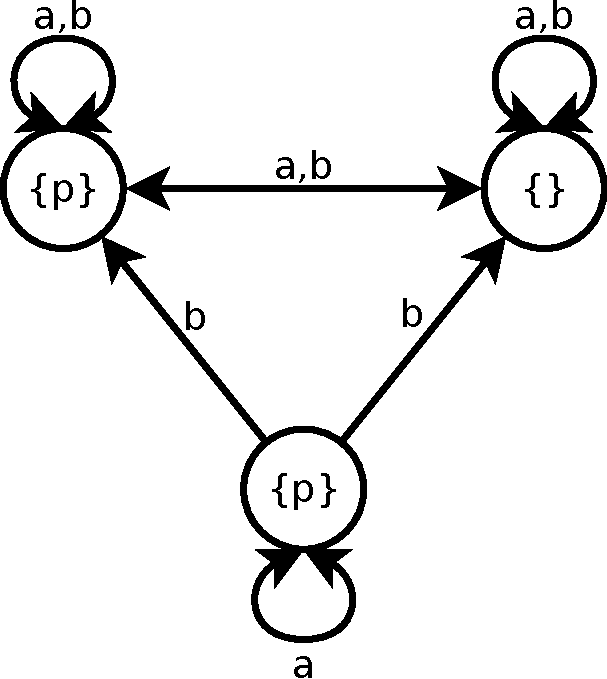
\includegraphics{semantics-coin-kd45}
}
\caption{\label{semantics-coin-kd45-1}
After Alice looks at the coin, she can distinguish between the worlds where the
coin lands on heads or tails, but Bob still cannot distinguish between these
worlds, and neither does he know that Alice can. The actual world is the world
on the bottom.
}
\end{center}
\end{figure}

We note that the statement is not satisfied in the setting of epistemic logic.
This should be clear, as in an epistemic setting, if Alice knows that the coin
landed on heads, then Bob cannot know that this isn't the case, because in an
epistemic setting agents can only know statements that are actually true.
\end{example}

We briefly list some properties of the refinement quantified modal logic, to
give some intuition about the logic. 
\pagebreak
\begin{proposition}
We have the following validities: 
\begin{enumerate}
\item $\entails_{\logicKF} \allrefs_a (\phi \implies \psi) \implies \allrefs_a
\phi \implies \allrefs_a \psi$
\item $\entails_{\logicKF} \allrefs_a \phi \implies \phi$
\item $\entails_{\logicKF} \allrefs_a \phi \implies \allrefs_a \allrefs_a \phi$
\item $\entails_{\logicKF} \phi$ implies $\entails_{\logicKF} \allrefs_a \phi$
\item $\entails_{\logicKF} \knows_a \allrefs_a \phi \implies \allrefs_a \knows_a
\phi$
\end{enumerate}
\end{proposition}

These properties were shown by van Ditmarsch and
French~\cite{french2009simulation}. We note that these properties are also valid
in \logicSF{} and \logicKDF{}.

In previous work, van Ditmarsch, French and Pinchinat~\cite{french2010future}
have considered the refinement quantified modal logic, \logicKF{}, based in the
class of models \classK{}. They provided a sound and complete axiomatisation for
the single-agent case, showed that it was expressively equivalent to the
single-agent modal logic, gave a decision procedure for the single-agent case
that runs in 2EXP time, and showed that the refinement quantified modal logic is
exponentially more succinct than the refinement quantified modal logic.

In this paper we move towards other variants of refinement quantified modal
logics, including the single-agent refinement quantified epistemic and doxastic
logics, and the multi-agent refinement quantified modal and doxastic logics. We
provide sound and complete axiomatisations for each of these logics, and show
that they are expressively equivalent to the modal logics that they are based
on. The expressivity result in particular allows us to show several results for
each of these logics, particularly that they are all decidable.
